\documentclass[./main.tex]{subfiles}

\begin{document}

\chapter{Introduction}\label{chapter:introduction}

"Only what is evolving is alive" \footnote{Pierre Kerner translation from french, original quote "N'est vivant que ce qui évolue"} this definition of life, like many others, is incomplete and we can probably find some corner case. This definition is based on the definition of evolution. We can try to define the evolution of a thing as the change on the thing to optimize its capability to conserve itself. To do that a thing need a memory.

In the majority of current know life, the physical support of this memory was DNA for DeoxyriboNucleic Acid. DNA is a molecule composed of two strains. Each strain is composed of a phosphate backbone. Along these backbones, we have a sugar linked to a nucleic acid. We have four types of nucleic acid: Adenine (A), Thymine (T), Cytosine (C) and Guanine (G), Figure \ref{intro:fig:dna_rna_pres} shows the 3d structure of DNA.

The two strands of DNA are linked by their nucleic acids, with some rules. In front of an, A we will always have a T, in front of a C we will always have a G and inside out. A DNA strain is a complementary of the other. But we cannot add a new DNA base to each DNA strain at the same end, for some of chemical properties that we will not detail here. We say DNA is composed of two anti-parallel strains. By convention we always represent DNA in the same orientation.

In bioinformatics, we generally represent a DNA strain by a single string on a four letter alphabet (A, C, T, G). The properties described above allow us to reconstruct the composition of one strand from the other by using the complementary letters (replace A by T, T by A, C by G and G by C) and reverse the order.%AL %JSV

\begin{figure}[ht]
    \centering
    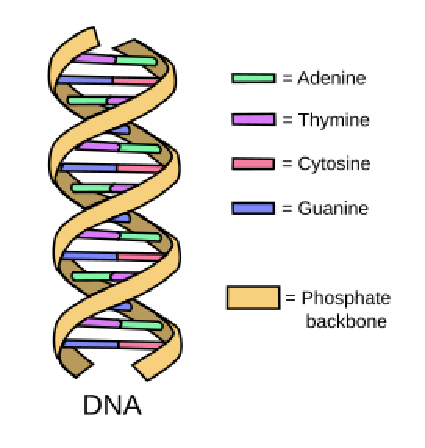
\includegraphics[width=5cm]{introduction/images/DNA.pdf}
    \caption{Structure and composition of DNA. Source: Wikipedia \protect\url{https://en.wikipedia.org/wiki/File:DNA_simple2.svg}}
    \label{intro:fig:dna_rna_pres}
\end{figure}

With many complex mechanisms, not detailed here, information contained in DNA is used to build essential molecules to keep the organism alive and reproduce it.%AL
This information is therefore the basis of the organism's functioning. If this information is destroyed or modified, the living organism will behave differently or die. Thus, knowing and understanding the succession of DNA bases is therefore (but not the only one) an effective entry point for analyzing many biological phenomena, diseases, evolution,… % JSV

To read this information, we rely on many biochemical techniques that we group under the term sequencing techniques. These techniques allow to read fractions of DNA fragments more or less long and with a variable error rate.%AL %JSV

\section{Sequencing} \label{section:introduction:sequencing}

Sequencing technologies evolved quickly since 1977\cite{sanger_sequencing}. Today we distinguish three generations of sequencing technologies, based on their properties.
In this section we focus on sequencing technologies properties and their impact on different bioinformatics tasks and do not detail the underlying biochemical methods.%AL

The two most important properties of a sequencing technology are the size of the DNA fragments it can read expressed in number of bases and also the number of errors that the technology will produce expressed in percentage. An error rate of 0.1\% indicates that the sequencer will make one error every thousand bases.
When sequencing can read large fragments we have more information about the original sequence, which facilitates downstream analysis.
If a read contains many errors (replace a letter by an other one, insert random data or skip a part of data), use information provide by sequencing tools may be impossible or require additional operations which will sometimes be very expensive (in terms of computer time).

\begin{table}[ht]
    \centering
    \begin{tabular}{ll|rr|l}
Generation & Technology          & Read length (bd)                 & Error rate             & Source                          \\ \hline
Second     & ABI/Solid           & 75                               & Low ($\approx$ 2\%)    & \cite{seq_assembly_demystified} \\
Second     & Illumina/Solexa     & 100–150                          & Low ($<$2\%)             & \cite{seq_assembly_demystified} \\
Second     & IonTorrent          & $\approx$ 200                    & Medium ($\approx$ 4\%) & \cite{seq_assembly_demystified} \\
Second     & Roche/454           & 400–600                          & Medium ($\approx$ 4\%) & \cite{seq_assembly_demystified} \\
First      & Sanger              & $\approx$ 2 kb                   & Low ($\approx$ 2\%)    & \cite{seq_assembly_demystified} \\
Third      & Pacific Biosciences & $\approx$ 10 kb ($\max$ 100 kb)  & High ($\approx$ 18\%)  & \cite{seq_assembly_demystified} \cite{longread_dark_matter} \\
Third      & Oxford Nanopore     & $\approx$ 10 kb ($\max$ 1 mb)    & High ($\approx$ 12\%)  & \cite{longread_dark_matter} \cite{nanopore_read_accuracy} \\
    \end{tabular}
    \caption{This table presents length of reads and error rate of main sequencing technology. Pacific Biosciences and Oxford Nanopore evolve quickly and different papers may report diverse figures.
    .}
    \label{intro:tab:technology_property}
\end{table}

Sanger technique produces long reads with very small error rate, but with a very low throughput and a very expensive cost per base. %AL
Second generation appeared in the mid-2000s. It increased the throughput and reduced the cost per base, but reduced dramatically the length of the reads and increases the probability of error ($\approx$ 1\%).%by orders of magnitude
The most frequent error type for this technology is a substitution between two nucleotides, (i.e. sequencer reads \texttt{A} in place of a \texttt{T}).%AL
Third generation dates back to the early 2010s. It has greatly increased the size of the reads but also the error rate while maintaining a good throughput. %decent ?
Errors in third generation are mostly insertion or deletion, sequencer didn't read a part of sequence or introduce random base not present in original sequence. Table \ref{intro:tab:technology_property} present read length and error rate on many sequencing technology.%AL
We would like to emphasize that both second and third generation technologies are always used today, and sometimes both technologies are used for a single experiment, as we will discuss later about hybrid techniques. %JSV

\jsv{je pense que cette phrase est inutile : DNA sequencing is very useful tools for many analysis, and in some cases is mandatory to be able to understand biological mechanisms.} %AL

With sequencing one can read all information contains in a genome. But, no matter the technology, we get lots of (short) unordered fragments. Genome assembly therefore designate the task of reconstructing the original sequence from this set of unordered fragments.%AL

\section{The genome assembly task}

If you want study an organism, knowing the complete genome sequence is very useful for a lot of task as finding 
genes of interest or study the sequence variations across a population \ldots.%AL
Yet, the best sequencing technologies still provide reads that are at least 2 orders of magnitude shorter than the genome. To understand the assembly problem, we provide a useful analogy which, to the best of our knowledge, has never been formulated before.

Imagine a crazy copyist monk. He is copying a book but he randomly chooses where he starts to copy, and he only copies small fragments of text at a time.
The copyist monks make errors, e.g. he would sometimes replace a symbol by another one, would skip a symbol, or would add a random symbol. We respectively call these errors substitutions, deletions and insertions.
Now imagine that there are multiple such copyist monks.
They choose randomly where they begin to write. They can choose several times the same region of the book or never choose to copy a certain region.
We refer by "coverage" the number of times a given chunk of the original book is copied. Coverage may significantly differ across the genome's regions.%AL
In this analogy, the book is the genome of the organism we want to study, and the copyist monks are our sequencer. The fragments of text are reads, and the operation to rebuild the book is assembly.

The assembly task can be seen as an ordering problem.%AL 
We try to put the text fragments in the original book order, and merge common parts at the end.%AL

To carry out this ordering, we can randomly take a fragment of text and search among all the others which begins by the end of the our fragment, the prefix of the second fragment corresponds to the suffix of the first fragment. When we observe this phenomenon we say that the fragments overlap. This a key concept in assembly. Once we have found the best overlap (generally the longest) for a text fragment we can merge the two fragments into one and restart our search for a new fragment that overlaps with the one we just created. And so on until there is no more fragments. This presentation of assembly task is very simple and we will see in more details some assembly algorithm details in chapter \ref{chapter:sota}.

%\section{Assembly glossary} 
\bigskip

Assembly community like any other scientific community create her own terms, to designate object they manipulate.%OULA
%
A \textbf{read} designate a fragment of DNA produced by sequencer.
%
A \textbf{overlap} ocurre between two reads when the suffix of a read is similar to the prefix of an other read. The length of this common part was the length of overlap.
%
A \textbf{contig} designates a sequence of DNA produced by an assembly tools. Exact definition of what is a \textbf{contig} changes between each assembly tool. We can see in some publication the term \textbf{unitig}. The only thing common in \textbf{unitigs} definition is that \textbf{contigs} are built from \textbf{unitigs}.
%
A \textbf{scaffold} designates an ordering of contigs. Most of the times we can't reconstruct each chromosome in one contig. We describe some reasons of this fragmentation later. But with external information such as restriction cards, linked reads or target sequencing, we can order contigs and determinate approximately the number of bases between them and become near to the real genome.%AL
%
Figure \ref{intro:fig:assembly} gives a summary of how reads are processed to obtain an assembly.
\begin{figure}[ht]
	\centering
	\pim{Add schéma to present each notion}
	\caption{Schematic of DNA assembly.}
    \label{intro:fig:assembly}
\end{figure}

\section{Thesis outline}


As stated above, latest sequencing technologies allows to sequence larger DNA fragments. One could think that the task of assembly becomes easier since we have to solve a puzzle with larger pieces. But this is not the case, as we will see in the following chapters. The main goal of this work is \jsv{a finir et a revoir}


Chapter \ref{chapter:preassembly} addresses steps performed before assembly. %AL
The  data quality  provided to the assemblers has a direct impact on the produced result.%AL
This chapter describes the state of the art of tools used to detect overlap between DNA fragments. The first contribution is a discussion on how to compare such tools (published as a blog post). 
The second contribution of the chapter is a paper that presents two tools we developed during this thesis \cite{yacrd}.
\yacrd  detects and removes regions with very high error rates in reads.
Experiments show that removing  low quality regions from reads improve assembly tools results.%AL
And \fpa which allows to filter out overlaps in order to focus on most informative ones.

Chapter \ref{chapter:sota} presents a state of the art of several assembly methods, both from a theoretical point of view and by presenting how some tools work in practice. This chapter introduces key concepts used in the next chapter.

Chapter \ref{chapter:postassembly} addresses the . The first contribution is a blog post that presents the difficulties of evaluating assembly tools that do not correct reads or even contigs. The second contribution 
 presents our tool for analyzing and improving assembly results, \knot that we developed during this thesis \cite{knot}.

Chapter \ref{chapter:other_contribution} will focus on my scientific contributions that could not be developed as a dedicated chapter: participation in the development of a graphical interface for genomic data analysis, participation in the CAMI2 contest, and some work around 10X data.

\onlyinsubfile{
\bibliographystyle{plainnat}
\bibliography{main}
\addcontentsline{toc}{chapter}{Bibliography}
}

\end{document}